%%sections like this
\section{Problem description}
\label{problem}

%%subsections like this
\subsection{Motor Schematics}

%%subsubsections like this
\subsubsection{Stator Assembly}

%%figures
\begin{figure}[ht]\begin{center}
 \fbox{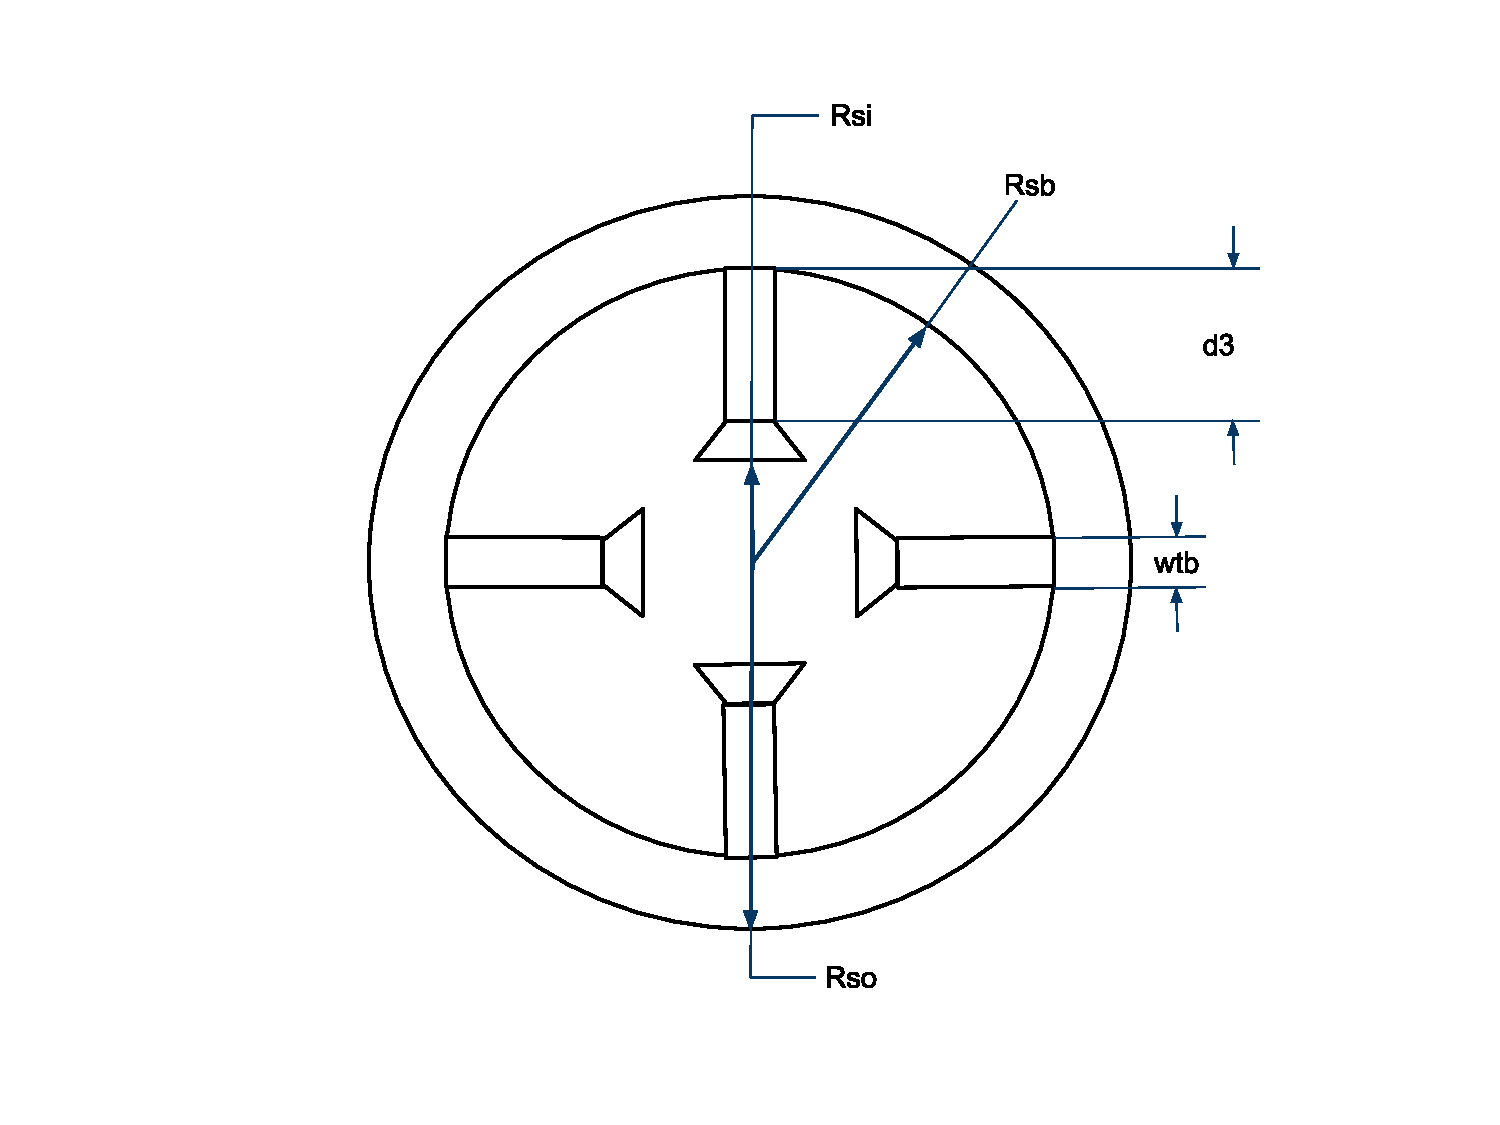
\includegraphics[width=100mm, height=75mm]{diagrams/bdcpmStator.eps}}
 \caption{BDCPMM Stator assembly}
 \label{bdcpmStator}
\end{center}\end{figure}


%%table
\begin{table}[!ht]
\centering
\begin{tabular}{|c|c|c|c|c|c|c|c|}
 \hline
 $L_{type}$ & $R_{si}$ (mm.) & $d_3$ (mm.) & $w_{tb}$ (mm.) & $w_{bi}$ (mm.) & $L_{cl}$ (mm.)& $R_{sh}$ (mm.) & $R_{st}$ (m) \\
 \hline
 X & 21.90 & 12.0 & 2.39 & 5.23 & 4.215 & 4.11 & 0.016 \\
 \hline
 Y & 22.22 & 15.1 & 2.39 & 5.23 & 4.265 & 4.11 & 0.016 \\
 \hline
 Z & 25.40 & 15.1 & 2.80 & 5.50 & 4.775 & 4.45 & 0.019 \\
 \hline
 \end{tabular}
\caption{Dimensions of the BDCPM motor family}
\label{ltypeDimTable}
\end{table}

%%multiple figures
\begin{figure}[ht]\begin{center}
 \subfloat[Isomap Residual Variance for the Pareto-front]{
 \label{isoRVbdcpmAll} \includegraphics[width=62mm, height=52mm]{diagrams/isoRVbdcpmAll.eps}}
 \subfloat[Explained variance for Principal Components of the Pareto-front]{
 \label{pcaEVbdcpmAll} \includegraphics[width=62mm, height=52mm]{diagrams/pcaEVbdcpmAll.eps}}
 \caption{Isomap and PCA results}
 \label{bdcpmmVar}
\end{center}\end{figure}
%%residual variance figure here
